\section{Logistic Regression (LR)} \label{sec:prob1}
In this section, we consider Logistic Regression (LR) for binary classification of several 2D datasets, and compare the effect of different model parameters and regularization.

\subsection{Part 1}
[todo]




\subsection{Part 2}
An alternative regularization ($L_1$) was then compared against $L_2$ from the previous section.
In~\cref{fig:1_2_all_weights_good}, the elements of the weight vector are compared.
The top row shows $L_1$ regularization for each of the four datasets, and the bottom row shows $L_2$.
In general, increased regularization parameter, $\lambda$, causes smaller magnitude weight vector, since the blue and green points (small $\lambda$) are further from zero than the magenta and yellow points (large $\lambda$).
This is true for both $L_1$ and $L_2$ regularization.
Especially clear in the 2nd and 4th columns, $L_1$ regularization creates a more sparse weight vector, as all elements are zero (yellow) for the highly regularized case, whereas with the same regularization constant with a $L_2$ penalty has some non-zero elements.

In addition to the weight vector, the decision boundary is affected by $\lambda$ and regularization method. 

Finally, the test-set classification error is also compared across $\lambda$ values and regularization methods.


\begin{figure}
	\centering
	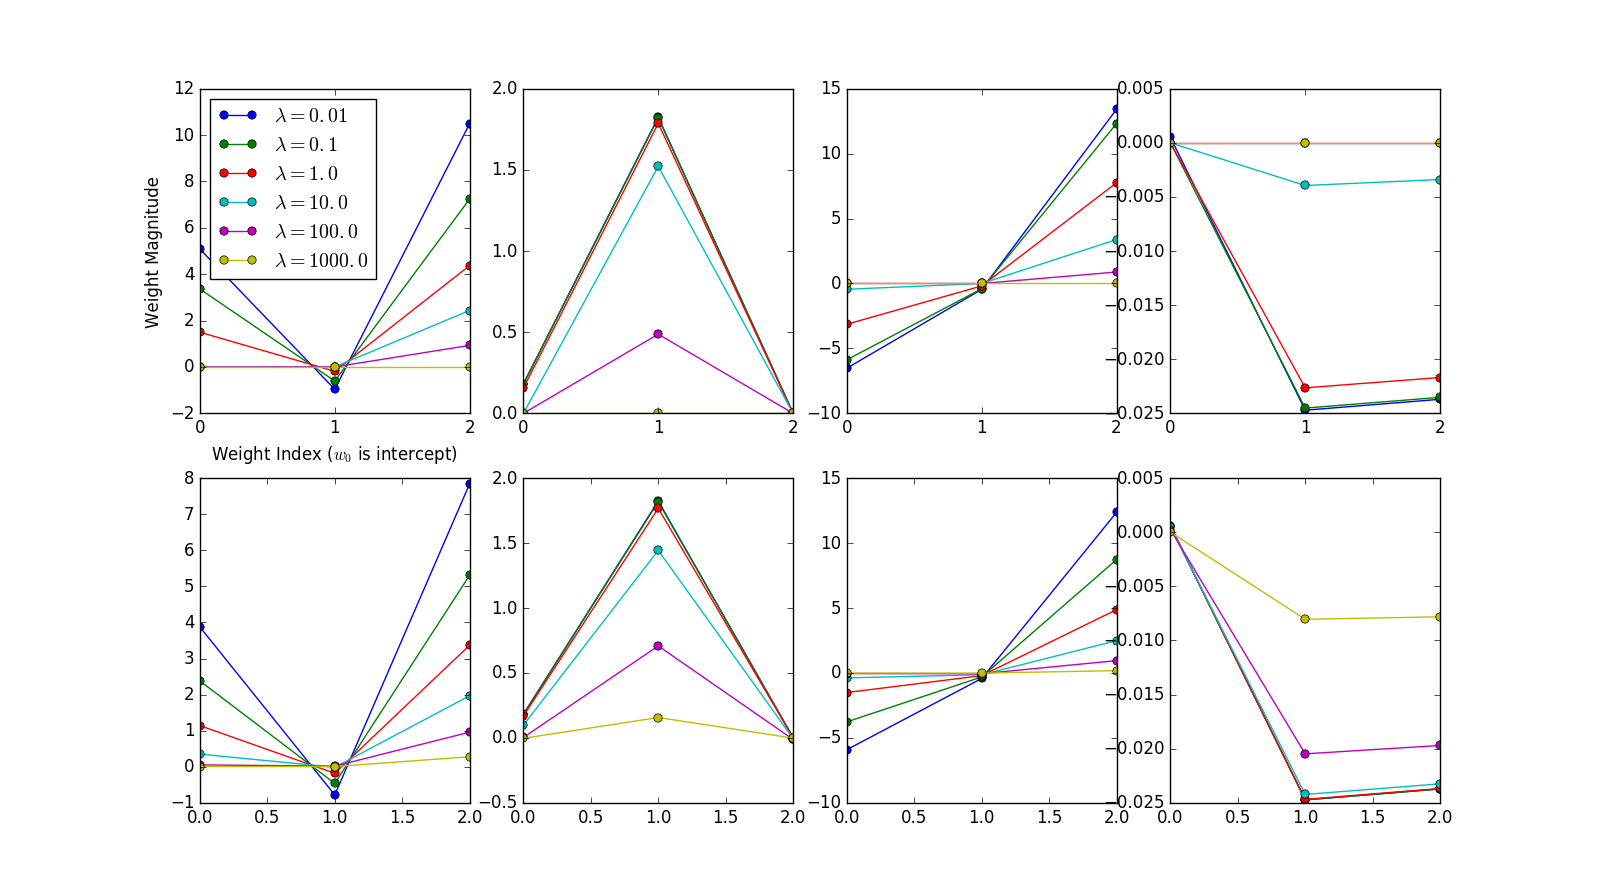
\includegraphics [trim=0 0 0 0, clip, angle=0, width=0.8\columnwidth,
	keepaspectratio]{figures/1_2_all_weights_good}
	\caption{Weight vectors of $L_1$ regularization (top row) and $L_2$ reg. (bottom row) for four datasets. Each column is the model for the same dataset. Within each subplot, several values of $\lambda$ are shown. For high lambda, weights are smaller in magnitude for all plots. $L_1$ reg causes sparser weight vector (more zero elements) than $L_2$.}
	\label{fig:1_2_all_weights_good} 
\end{figure}

\begin{figure}
	\centering
	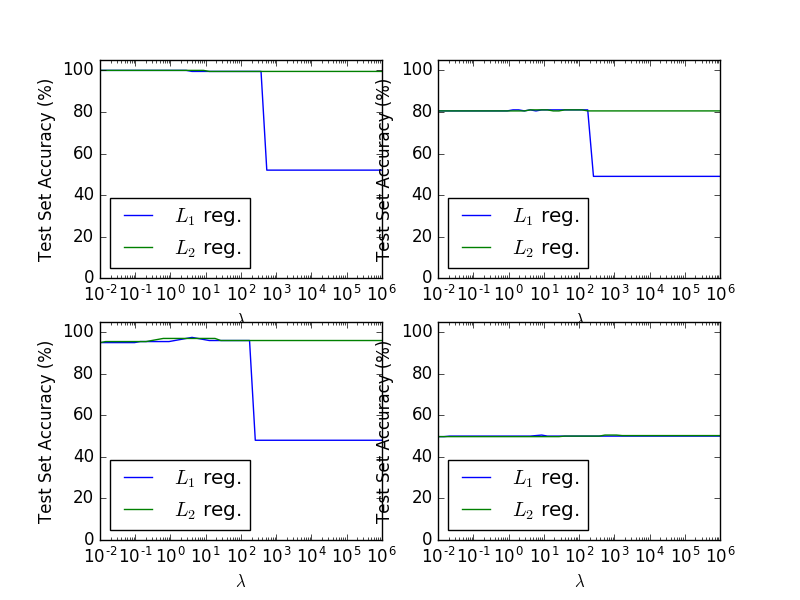
\includegraphics [trim=0 0 0 0, clip, angle=0, width=0.8\columnwidth,
	keepaspectratio]{figures/1_2_accuracy}
	\caption{} 
	\label{fig:1_2_accuracy} 
\end{figure}

\subsection{Part 3}
[todo]

